\documentclass[conference]{IEEEtran}
\IEEEoverridecommandlockouts
\usepackage{amsmath,amssymb}
\usepackage{booktabs}
\usepackage{array}
\usepackage{tabularx}
\usepackage{multirow}
\usepackage{graphicx}
\usepackage{cite}
\usepackage{url}
\usepackage{tikz}
\usetikzlibrary{arrows.meta,positioning,shapes.geometric,fit,backgrounds}
\usepackage{pgfplots}
\pgfplotsset{compat=1.18}
\usepackage{algorithmic}
\usepackage{xcolor}
\usepackage{enumitem}
\usepackage{microtype}

\title{
PhishSense: AI-Based Phishing Detection with Blockchain-Backed Threat Intelligence
}
\author{
\resizebox{\textwidth}{!}{%
\begin{tabular}{ccc}
\textbf{M. DHARMA TEJA} &
\textbf{BHEEMA NITISH GURU DATHA} &
\textbf{GAJJALA CHARITHA} \\[2pt]


Department of CSE &
Department of CSE &
Department of CSE \\

Vel Tech Rangarajan Dr. Sagunthala R\&D &
Vel Tech Rangarajan Dr. Sagunthala R\&D &
Vel Tech Rangarajan Dr. Sagunthala R\&D \\

Institute of Science and Technology &
Institute of Science and Technology &
Institute of Science and Technology \\

Chennai, India &
Chennai, India &
Chennai, India \\

\textit{dharmatejamd@gmail.com} &
\textit{nitishbheema@gmail.com} &
\textit{charithagajjala1@gmail.com}
\end{tabular}%
}
}

\begin{document}

\maketitle


% ─────────────────────────────────────────────────────────────────────────────
% ABSTRACT
% ─────────────────────────────────────────────────────────────────────────────
\begin{abstract}
Phishing has grown far beyond the spoofed e-mails and look-alike URLs of earlier decades.
Today's threat actors craft dynamically rendered login pages, hide malicious links inside
QR codes distributed on physical posters and social media, and engineer the browsing experience
itself to manipulate victims before any credential is entered.
Conventional defenses---URL blacklists, lexical classifiers, and even screenshot-based visual
detectors---operate on a single signal and therefore fail the moment an adversary shifts
strategy.

This paper presents \textit{PhishSense}, a unified, domain-independent digital threat detection
platform that deliberately fuses several independent evidence channels: lexical URL analysis,
QR code destination decoding and analysis, HTML/DOM structural inspection, real-time user
behavioral fingerprinting, AI/ML classification, SHAP-style explainability, similarity-based
campaign attribution, an adaptive multi-stage risk engine, and a blockchain-backed tamper-evident
threat intelligence ledger.
The system is intentionally modular so that each channel can be studied and evaluated
independently, yet all channels feed a single risk score with an attached natural-language
explanation.

PhishSense is implemented on a full production-grade stack: a React~18 frontend with a
built-in behavioral event tracker, a Spring Boot~3 API gateway, a Python FastAPI AI
service, a PostgreSQL database for session history and security alerts, a custom
proof-of-work blockchain module for threat logging, and an HMAC-SHA256 JWT authentication
layer supporting Google OAuth and email OTP.
This paper describes the complete architecture, feature engineering rationale, mathematical
model, evaluation protocol, and ablation plan.
Performance tables are provided as experimental templates; no accuracy figures are fabricated.
\end{abstract}

\begin{IEEEkeywords}
phishing detection, behavioral analytics, machine learning, explainable AI, threat intelligence,
blockchain, QR phishing, cybersecurity, threat fingerprinting, adaptive risk scoring.
\end{IEEEkeywords}

% ─────────────────────────────────────────────────────────────────────────────
% I. INTRODUCTION
% ─────────────────────────────────────────────────────────────────────────────
\section{Introduction}

Phishing is not a solved problem.
Despite decades of research and deployment of increasingly sophisticated defenses, it remains one
of the most economically damaging threat vectors in existence.
The Anti-Phishing Working Group documented record attack volumes in 2023, with threat actors showing
a clear shift toward techniques that are designed specifically to defeat URL-based
detection~\cite{ref1,ref2}.

The earliest defenses were blacklists: when a phishing URL was reported, it was added to a list
that browsers and mail gateways queried.
The problem is obvious---a URL must be seen and reported before it is blocked, a gap that is
typically measured in hours to days~\cite{ref3}.
Machine-learning classifiers over URL features closed some of that gap by allowing novel URLs to
be scored before they were reported~\cite{ref4,ref5}.
But URL feature classifiers can be deliberately defeated: an attacker who knows which lexical
features a model uses can construct a URL that scores ``legitimate'' while the page behind it
harvests credentials~\cite{ref6}.
This family of attack---sometimes called feature evasion or adversarial URL crafting---has been
documented repeatedly in the literature.

Webpage-level analysis goes deeper, examining HTML structure, embedded scripts, and the visual
appearance of the rendered page~\cite{ref7,ref8,ref9}.
These approaches are harder to evade because modifying the page's DOM structure is more expensive
than tweaking a URL string.
However, they still miss a critical dimension: the experience the page creates for the victim
through timed redirects, fake loading screens, scripted focus events, and behaviorally engineered
urgency cues.
A page that appears clean in a static DOM snapshot may behave maliciously the moment a user
begins to interact with it.

A separate and rapidly growing attack surface is \textit{quishing}---phishing delivered through
QR codes~\cite{ref10}.
A QR code printed on a flyer, embedded in a PDF, or sent as an image bypasses every URL-based
filter in email gateways and browser extensions.
The destination URL is invisible until decoded by a camera, and by that point the user is
already navigating toward the threat.

Finally, most threat intelligence today lives in centralized repositories whose contents are
difficult to verify for integrity, expensive to access across organizational boundaries, and
updated at human timescales~\cite{ref11}.
An organization that detects a novel phishing campaign cannot efficiently share that knowledge
in a form that other systems can trust and act on automatically.

\textit{PhishSense} was built to address all four of these gaps together.
Rather than being the first system to use any one technique, its contribution is the
\textit{integration and evaluation of multiple complementary detection channels}---URL analysis,
QR decoding, DOM inspection, user behavioral fingerprinting, AI/ML classification, explainable AI,
similarity-based campaign attribution, adaptive risk scoring, and blockchain-backed threat
intelligence---in a single cohesive, domain-independent framework.
No single channel can be fooled while the others remain uninformed.

The specific contributions of this work are:
\begin{enumerate}[leftmargin=*,nosep]
\item A \textit{multi-modal input pipeline} that processes URL strings, QR code images, live
      webpage content, and user behavioral sessions as four complementary input channels within
      one analysis graph.
\item A \textit{behavioral fingerprinting module} that captures interaction signals---click
      latency, mouse movement entropy, keystroke timing, form-focus behavior---and converts them
      into a normalized session fingerprint for anomaly detection.
\item An \textit{adaptive risk engine} that accumulates evidence from each analysis stage and
      updates a continuous risk score rather than producing one static label.
\item A \textit{threat fingerprinting and similarity search module} that identifies whether a
      newly observed URL shares structural or behavioral lineage with a known campaign, enabling
      early detection of zero-day variants.
\item A \textit{blockchain-backed threat intelligence ledger} that logs confirmed threat
      fingerprints as tamper-evident records that can be reused across sessions without storing
      any personally identifiable information on-chain.
\item A \textit{SHAP-style explainability layer} that attaches a ranked, plain-language evidence
      list to every decision, letting a non-expert user understand \textit{why} a resource was
      flagged.
\end{enumerate}

% ─────────────────────────────────────────────────────────────────────────────
% II. RELATED WORK
% ─────────────────────────────────────────────────────────────────────────────
\section{Related Work}

\subsection{URL and Machine-Learning Based Detection}
The most extensively studied approach to phishing detection uses features extracted from the URL
string alone---length, subdomain depth, special characters, entropy, and suspicious token
presence.
Sahingoz et al.\ evaluated seven classifiers including Random Forest, SVM, and neural networks
on this feature space and found Random Forest to be the strongest~\cite{ref4}.
Mohammad et al.\ combined URL heuristics with page-level signals and reported strong results on
a balanced benchmark~\cite{ref5}.
Basit et al.\ surveyed deep-learning extensions of this line and identified adversarial evasion
and class imbalance as the two most persistent challenges that the URL-feature paradigm has not
fully solved~\cite{ref6}.
The lesson from this body of work is that URL features are fast and effective on known attack
patterns but brittle when an attacker specifically optimizes against them.

\subsection{Webpage and Visual Analysis}
Going beyond the URL, Abdelnabi et al.\ introduced VisualPhishNet, which compares page screenshots
to a registry of protected brand logos using few-shot visual similarity~\cite{ref7}.
This approach is harder to evade because cloning a brand's visual identity requires more effort
than changing a URL, but it still depends on maintaining an up-to-date brand registry and does
not capture dynamic behavior.
Lin et al.\ incorporated HTML structure and JavaScript behavior into the feature space~\cite{ref8},
and Marchal et al.\ analyzed DOM-level signals such as form attributes, iframe counts, and
external resource ratios~\cite{ref9}.
These works improve detection of visual cloning attacks but assume that the malicious behavior
is present in the static page snapshot, which is not always true for pages that activate their
harvesting logic only after detecting user interaction.

\subsection{Dynamic and Behavioral Analysis}
Canali et al.\ analyzed malicious web pages using dynamic execution traces---observing what scripts
the page executes, what network calls it makes, and what DOM modifications it triggers
during rendering~\cite{ref12}.
Cova et al.\ used similar dynamic script features to detect exploit kits~\cite{ref13}.
These are page-execution-level behavioral approaches; they observe what the \textit{page does},
not what the \textit{user does}.
PhishSense extends this line by treating the victim's interaction pattern as an independent
evidence channel: how quickly a user types into a credential field, whether they hesitate or
backspace, and how their mouse moves over a form element are signals that a legitimately
experienced user produces differently than a victim who is confused by a fake page.

\subsection{QR Code Phishing}
Kharraz et al.\ documented the use of QR codes as a phishing delivery vector and showed that
conventional URL scanners are architecturally blind to QR-encoded destinations~\cite{ref10}.
A QR image is opaque to a text-based filter; only a camera and a decoder reveal the destination.
PhishSense adds a dedicated QR analysis module that decodes the payload and subjects the
destination to the full threat pipeline before any navigation occurs.

\subsection{Explainable AI for Security}
Lundberg and Lee introduced SHAP (SHapley Additive exPlanations), a theoretically grounded
framework for attributing predictions to individual input features~\cite{ref15}.
Marino et al.\ applied XAI to network intrusion detection and showed that operators are more
likely to trust and act on detections when they can see which features drove a decision~\cite{ref16}.
This is particularly important for a phishing detector: a user who sees only a risk score has
no actionable information, while a user who sees ``flagged because of credential-harvesting form
+ suspicious redirect + fingerprint match to Campaign~\#7'' can make an informed decision.

\subsection{Blockchain for Threat Intelligence Sharing}
Traditional threat intelligence feeds are centralized, require trust in the feed provider, and
cannot be independently verified.
Al-Riyami and Paterson laid cryptographic foundations for distributed trust~\cite{ref11}.
Alexopoulos et al.\ built a prototype blockchain-backed platform for sharing
indicators-of-compromise and measured its operational overhead~\cite{ref17}.
PhishSense adopts a lightweight local proof-of-work chain that logs confirmed threat fingerprints
in a tamper-evident structure, enabling intelligence reuse within and across sessions without
depending on any external feed or central server.

\begin{table}[!t]
\caption{COMPARATIVE SUMMARY OF RELATED APPROACHES}
\label{tab:lit}
\centering
\scriptsize
\setlength{\tabcolsep}{2pt}
\begin{tabularx}{\columnwidth}{|>{\raggedright\arraybackslash}p{0.19\columnwidth}|>{\raggedright\arraybackslash}p{0.13\columnwidth}|c|c|c|c|>{\raggedright\arraybackslash}X|}
\hline
\textbf{Approach} & \textbf{Input} & \textbf{ML} & \textbf{Behav.} & \textbf{XAI} & \textbf{Chain} & \textbf{Key limitation} \\ \hline
Sahingoz~\cite{ref4}       & URL+HTML      & \checkmark &            &            &            & Evasion by URL crafting \\ \hline
VisualPhishNet~\cite{ref7} & Screenshot    & \checkmark &            &            &            & Needs brand registry \\ \hline
Canali~\cite{ref12}        & Script trace  & \checkmark & \checkmark &            &            & Page-level only, no user signals \\ \hline
Kharraz~\cite{ref10}       & QR/URL        & \checkmark &            &            &            & No page or behavioral analysis \\ \hline
Alexopoulos~\cite{ref17}   & IoC hash      &            &            &            & \checkmark & No ML, no detection layer \\ \hline
\textbf{PhishSense (ours)} & URL+QR+DOM+Behav. & \checkmark & \checkmark & \checkmark & \checkmark & See Section~\ref{sec:limits} \\ \hline
\end{tabularx}
\end{table}

% ─────────────────────────────────────────────────────────────────────────────
% III. PROBLEM STATEMENT, REQUIREMENTS, AND OBJECTIVES
% ─────────────────────────────────────────────────────────────────────────────
\section{Problem Statement, Requirements, and Objectives}

\subsection{Formal Problem Statement}
Let an \textit{input event} $\mathcal{I}$ be a tuple $(u, q, w, b)$, where $u$ is an optional
URL string, $q$ is an optional QR image, $w$ is an optional webpage DOM snapshot, and $b$ is an
optional behavioral session trace.
Any of the four components may be absent depending on what the user provides.
The detection task is to learn a function
\begin{equation}
  f : \mathcal{I} \;\rightarrow\; \{0,1\} \;\times\; [0,1]
\end{equation}
that jointly produces a binary threat label $\hat{y}\in\{0,1\}$ and a calibrated risk score
$\hat{r}\in[0,1]$.
The label value~0 indicates a legitimate resource; value~1 indicates phishing or malicious.
Critically, $f$ must be \textit{domain-independent}: it must produce reliable outputs without
consulting URL blacklists, brand registries, or any database of previously seen URLs.
This constraint forces the model to reason from structure and behavior rather than from memory.

\subsection{System Requirements}
Table~\ref{tab:req} maps each high-level requirement to the design decision that implements it
and to the verification criterion used during evaluation.

\begin{table}[!t]
\caption{PHISHSENSE SYSTEM REQUIREMENTS}
\label{tab:req}
\centering
\scriptsize
\setlength{\tabcolsep}{3pt}
\begin{tabularx}{\columnwidth}{|>{\raggedright\arraybackslash}p{0.21\columnwidth}|>{\raggedright\arraybackslash}X|>{\raggedright\arraybackslash}p{0.22\columnwidth}|}
\hline
\textbf{Requirement} & \textbf{How it is met} & \textbf{Verification} \\ \hline
Multi-modal input      & URL, QR, DOM, behavioral pipeline   & Per-modality unit tests   \\ \hline
Domain independence    & No blacklist or brand registry used & Zero-day holdout split    \\ \hline
Behavioral analysis    & 13 session-level interaction features & Behavioral ablation       \\ \hline
Explainability         & SHAP-style ranked feature attribution & Human-readable audit log  \\ \hline
Adaptive risk scoring  & Evidence-accumulation across pipeline stages & Staged risk trace   \\ \hline
Threat fingerprinting  & Normalized projection of stable features & Fingerprint match rate \\ \hline
Similarity search      & Cosine nearest-neighbor against ledger index & Campaign F$_1$      \\ \hline
Blockchain integrity   & SHA-256 Merkle-chained proof-of-work blocks & Chain re-validation  \\ \hline
Privacy                & No PII or raw URLs stored on-chain  & On-chain schema audit     \\ \hline
Reproducibility        & Fixed seeds, dataset hashes, config manifests & Re-run output match \\ \hline
\end{tabularx}
\end{table}

\subsection{Research Objectives}
Three objectives drive the experimental design.
First, to build and validate a multi-modal feature pipeline that extracts complementary signal
from whichever input modalities are present.
Second, to train and evaluate AI/ML classifiers on the combined feature space and attach
SHAP-style explanations to every decision.
Third, to measure through controlled ablation how much each module---URL features, DOM features,
behavioral features, threat intelligence, blockchain reuse, adaptive risk, and similarity
search---independently contributes to detection performance.

% ─────────────────────────────────────────────────────────────────────────────
% IV. THREAT MODEL
% ─────────────────────────────────────────────────────────────────────────────
\section{Threat Model}

The adversary is an external attacker whose goal is to harvest credentials or deliver malware
by making a malicious resource appear legitimate.
We assume the attacker has the following capabilities.

\noindent\textit{URL manipulation.}
The attacker can register domains and subdomains with valid TLS certificates and can construct
URL strings whose lexical features score below classifier thresholds through typosquatting,
URL shortening, and deliberate selection of innocuous path tokens.

\noindent\textit{Visual and DOM cloning.}
The attacker can replicate the HTML/CSS/JavaScript structure of well-known legitimate pages and
can inject credential-harvesting forms that are visually indistinguishable from their targets.

\noindent\textit{QR delivery.}
The attacker can encode malicious URLs in QR images and distribute them through physical media,
social platforms, or e-mail attachments, bypassing URL-based filters entirely.

\noindent\textit{Behavioral evasion.}
The attacker knows that behavioral detectors exist and may attempt to add artificial timing delays
or simulate human-like mouse movement to suppress behavioral anomaly scores.

\noindent\textit{System assumptions.}
The analysis sandbox can safely fetch and render target URLs in isolation.
Behavioral signals are captured client-side before any credential is submitted.
The local blockchain node is trusted; no external consensus is required for threat logging.
The attacker does not have access to model parameters, feature thresholds, or the threat
fingerprint index.

The threat model explicitly excludes server-side credential compromise, physical device access,
and insider attacks.

% ─────────────────────────────────────────────────────────────────────────────
% V. PROPOSED SYSTEM ARCHITECTURE
% ─────────────────────────────────────────────────────────────────────────────
\section{Proposed System Architecture}

\begin{figure}[!t]
\centering
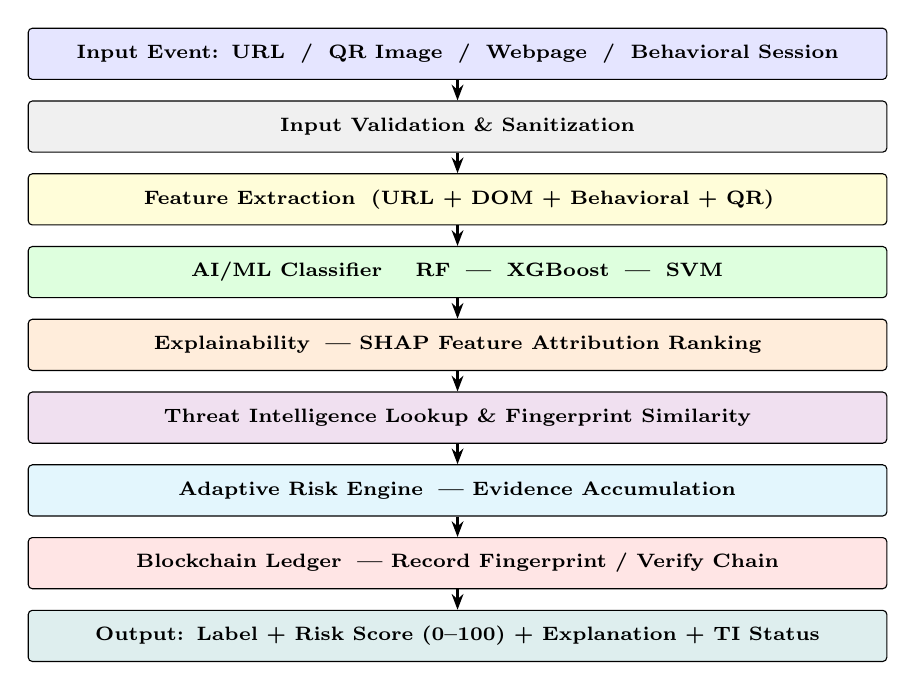
\begin{tikzpicture}[
  node distance=2.6mm,
  box/.style={draw, rounded corners=1.5pt, text width=0.88\columnwidth,
              align=center, minimum height=6.5mm, font=\scriptsize\bfseries},
  arr/.style={-{Stealth[length=2mm]}, thick}
]
\node[box, fill=blue!10]    (inp)   {Input Event: URL \;/\; QR Image \;/\; Webpage \;/\; Behavioral Session};
\node[box, fill=gray!12,  below=of inp]  (val)   {Input Validation \& Sanitization};
\node[box, fill=yellow!15,below=of val]  (feat)  {Feature Extraction \;(URL + DOM + Behavioral + QR)};
\node[box, fill=green!13, below=of feat] (ml)    {AI/ML Classifier \quad RF \;|\; XGBoost \;|\; SVM};
\node[box, fill=orange!14,below=of ml]   (xai)   {Explainability \;--- SHAP Feature Attribution Ranking};
\node[box, fill=violet!12,below=of xai]  (ti)    {Threat Intelligence Lookup \& Fingerprint Similarity};
\node[box, fill=cyan!11,  below=of ti]   (risk)  {Adaptive Risk Engine \;--- Evidence Accumulation};
\node[box, fill=red!10,   below=of risk] (chain) {Blockchain Ledger \;--- Record Fingerprint / Verify Chain};
\node[box, fill=teal!13,  below=of chain](out)   {Output: Label + Risk Score (0--100) + Explanation + TI Status};
\foreach \a/\b in {inp/val, val/feat, feat/ml, ml/xai, xai/ti, ti/risk, risk/chain, chain/out}
  \draw[arr] (\a) -- (\b);
\end{tikzpicture}
\caption{PhishSense end-to-end analysis pipeline.  Modules are independently testable;
all feed a single unified output.}
\label{fig:arch}
\end{figure}

Fig.~\ref{fig:arch} shows the complete pipeline.
Every input event enters an \textit{Input Validation} stage that sanitizes strings, resolves QR
payloads using a ZXing-compatible decoder, and sets a modality bitmask that tells each downstream
stage which sub-extractors to activate.
This single-entry-point design means that a URL scan, a QR scan, and a full behavioral session
all follow the same processing graph; the difference is which feature columns are populated.

The \textit{Feature Extraction} stage runs four parallel sub-extractors.
The URL extractor operates on the raw string without fetching the target.
The DOM extractor fetches the page and parses the HTML tree; for JavaScript-heavy pages a
Selenium-based sandbox is used.
The behavioral extractor reads the session event buffer accumulated by the React client-side
tracker.
The QR extractor decodes the payload and then reuses the URL and DOM extractors on the destination.
All four sub-vectors are $\ell_2$-normalized and concatenated before being passed to the classifier.

The \textit{AI/ML Classifier} produces a probability distribution over three classes:
Legitimate, Suspicious, and Phishing.
The \textit{Explainability} module decomposes that probability into per-feature SHAP attributions.
The \textit{Threat Intelligence Lookup} queries an in-memory index of fingerprints derived from the
blockchain ledger and returns the nearest-neighbor distance and campaign identifier.
The \textit{Adaptive Risk Engine} fuses classifier evidence, intelligence match strength, and
behavioral anomaly score into a single integer risk score on a 0--100 scale.
If that score exceeds a configurable threshold, the \textit{Blockchain Ledger} module generates a
new block containing the threat fingerprint hash and appends it to the local chain.
The final output bundles the threat label, risk score, ranked explanation, fingerprint hash, and
intelligence status into a structured JSON response that is displayed on the React client.

% ─────────────────────────────────────────────────────────────────────────────
% VI. FEATURE ENGINEERING
% ─────────────────────────────────────────────────────────────────────────────
\section{Feature Engineering}

Good features are the foundation of any detection system.
In PhishSense, features are organized into four groups that correspond to the four input
modalities, with a fifth group of intelligence features appended after the threat-lookup stage.

\subsection{URL Features (16 features)}
These are extracted from the raw URL string before any network request is made.
They include: URL character length; domain segment count; subdomain depth; presence of an IP
address in the host field; use of a known URL-shortening service; counts of special characters
(\texttt{@}, \texttt{-}, hyphens, dots); Shannon entropy of the host string; presence of
high-risk tokens such as \textit{login}, \textit{secure}, \textit{verify}, \textit{account},
and \textit{update}; redirect count in the query string; HTTPS presence; use of a non-standard
port; query string length; path depth; longest run of consecutive consonants; digit-to-character
ratio; and TLD risk class (high, medium, low).

\subsection{Webpage/DOM Features (11 features)}
These are extracted from the rendered HTML snapshot: count of \texttt{<form>} elements;
count of \texttt{<input type="password">} fields; count of external \texttt{<script>} tags;
count of hidden input fields; count of \texttt{<iframe>} elements; ratio of external to total
links; inline JavaScript byte length; presence of a \texttt{<meta http-equiv="refresh">} tag;
count of social-engineering keywords in visible text (\textit{urgent}, \textit{verify now},
\textit{account suspended}); external resource ratio; and absence of a matching favicon.

\subsection{Behavioral Features (13 features)}
These are derived from client-side interaction events without logging any content the user types.
Features include: mean and variance of inter-keystroke interval; click count within the first
ten seconds of page load; mouse movement path length; scroll depth ratio; form-focus event count;
rapid redirect count during the session; tab-switch count before first credential field focus;
time from page load to first password field interaction; typing-pause-to-typing ratio; backspace
frequency relative to total keystrokes; form submission attempt count; and navigation-event
entropy.

\subsection{QR Features (4 features)}
QR analysis inherits all URL and DOM features computed on the decoded destination, augmented by:
QR error-correction level (L/M/Q/H); QR version number; a flag indicating whether the decoded
URL differs from any anchor text visible near the QR image in its parent document; and a flag
indicating whether the parent document contains other suspicious signals independently.

\subsection{Threat Intelligence Features (3 features)}
After the threat-lookup stage, three features are appended: a binary flag for an exact
fingerprint match; the cosine similarity score to the nearest indexed fingerprint; and the
campaign cluster identifier of that nearest neighbor encoded as an ordinal integer.

% ─────────────────────────────────────────────────────────────────────────────
% VII. MATHEMATICAL MODEL
% ─────────────────────────────────────────────────────────────────────────────
\section{Mathematical Model}

\noindent\textbf{Feature representation.}
Let $\mathbf{x}_U\in\mathbb{R}^{d_U}$, $\mathbf{x}_D\in\mathbb{R}^{d_D}$,
$\mathbf{x}_B\in\mathbb{R}^{d_B}$, and $\mathbf{x}_Q\in\mathbb{R}^{d_Q}$ be the normalized
URL, DOM, behavioral, and QR sub-vectors respectively.
The full feature vector is their concatenation:
\begin{equation}
  \mathbf{x} = \mathrm{concat}\!\left(\mathbf{x}_U,\;\mathbf{x}_D,\;\mathbf{x}_B,\;\mathbf{x}_Q\right)
  \;\in\;\mathbb{R}^{d}
  \label{eq:feat}
\end{equation}
where $d = d_U + d_D + d_B + d_Q$.
Each sub-vector is $\ell_2$-normalized independently before concatenation to prevent large URL or
DOM feature magnitudes from dominating the lower-dimensional behavioral signal.

\noindent\textbf{Behavioral fingerprint.}
A session's behavioral fingerprint $\phi_B$ is a compact projection of the behavioral sub-vector:
\begin{equation}
  \phi_B = \frac{W_B\,\mathbf{x}_B}{\|W_B\,\mathbf{x}_B\|_2 + \epsilon}
  \label{eq:finger}
\end{equation}
where $W_B\in\mathbb{R}^{k\times d_B}$ is a learned projection matrix and $\epsilon$ provides
numerical stability.
A session whose fingerprint falls outside the benign behavioral envelope---defined by the
$k$-nearest neighbors from a held-out calibration split---contributes an elevated behavioral
anomaly score to the risk engine.

\noindent\textbf{Classifier output.}
The trained classifier maps the full feature vector to a probability distribution over three classes:
\begin{equation}
  P(y\mid\mathbf{x}) = \mathrm{softmax}\!\left(f_\theta(\mathbf{x})\right)
  \label{eq:cls}
\end{equation}
where $f_\theta$ is the learned model (Random Forest, XGBoost, or SVM) and
$y\in\{\text{Legitimate},\text{Suspicious},\text{Phishing}\}$.

\noindent\textbf{Threat fingerprint similarity.}
Given a new threat fingerprint $\phi$ and the nearest indexed fingerprint $\phi^*$, similarity is:
\begin{equation}
  s(\phi,\phi^*) = \frac{\phi \cdot \phi^*}{\|\phi\|\;\|\phi^*\|}
  \label{eq:sim}
\end{equation}
A similarity $s > \tau_{\mathrm{sim}}$ triggers a campaign attribution without requiring any URL
to have been previously seen.

\noindent\textbf{Unified risk score.}
The adaptive risk engine combines three evidence signals into a single score:
\begin{equation}
  R = \mathrm{clip}\!\left(100\cdot\bigl[\alpha\,P(\text{Phishing}\mid\mathbf{x}) +
       \beta\,s(\phi,\phi^*) + \gamma\,a_B\bigr],\;0,\;100\right)
  \label{eq:risk}
\end{equation}
where $a_B$ is the behavioral anomaly score, $\alpha+\beta+\gamma=1$, and $\mathrm{clip}(\cdot)$
bounds the output to the display range.
Weights are selected by validation-set search and frozen before any test evaluation.

\noindent\textbf{Adaptive risk update.}
As new evidence $e_k$ arrives during a live browsing session:
\begin{equation}
  R_{k+1} = \mathrm{clip}\!\left(R_k + \delta_k(e_k),\;0,\;100\right)
  \label{eq:adapt}
\end{equation}
The increment $\delta_k(e_k)$ is signed: detection of a credential-harvesting form pushes the
score upward; observation of a valid organization-name-matched TLS certificate pushes it slightly
downward.
This means the system never commits to a final decision prematurely.

\noindent\textbf{Blockchain block hash.}
Each confirmed threat record is committed to the chain as:
\begin{equation}
  H_k = \mathrm{SHA256}\!\left(H_{k-1} \;\|\; \mathrm{fp}_k \;\|\; t_k \;\|\; n_k\right)
  \label{eq:chain}
\end{equation}
where $H_{k-1}$ is the previous block hash, $\mathrm{fp}_k$ is the threat fingerprint hash,
$t_k$ is the Unix timestamp, and $n_k$ is the proof-of-work nonce.
The difficulty constraint on $H_k$ makes retroactive tampering computationally expensive.

% ─────────────────────────────────────────────────────────────────────────────
% VIII. MACHINE LEARNING MODELS
% ─────────────────────────────────────────────────────────────────────────────
\section{Machine Learning Models and Evaluation}

\subsection{Model Selection Rationale}
Four supervised classifiers are trained on the concatenated feature matrix of Eq.~\eqref{eq:feat}.
\textit{Logistic Regression} provides an interpretable linear baseline that clarifies what
performance is achievable without non-linearity.
\textit{Random Forest} captures feature interactions through an ensemble of unpruned decision
trees and is naturally resistant to irrelevant features.
\textit{Support Vector Machine with an RBF kernel} maximizes the margin in a high-dimensional
space, which is well suited to the mixed-type feature vector.
\textit{XGBoost} applies gradient-boosted trees with regularization and historically delivers
strong results on tabular cybersecurity datasets.
In addition, an \textit{Isolation Forest} is trained on the behavioral sub-vector alone to
support unsupervised anomaly detection for sessions that arrive without ground-truth labels.

\subsection{Training and Evaluation Protocol}
The dataset is split 70/10/20 into training, validation, and test partitions using stratified
sampling.
SMOTE oversampling addresses class imbalance within the training partition only; the validation
and test partitions are never resampled.
Hyperparameters are selected by five-fold cross-validation on training data.
The test partition is used exactly once for final metric reporting.

\begin{table}[!t]
\caption{CLASSIFIER PERFORMANCE --- TEMPLATE (POPULATE AFTER EVALUATION)}
\label{tab:models}
\centering
\scriptsize
\setlength{\tabcolsep}{3pt}
\begin{tabular}{|l|c|c|c|c|c|c|}
\hline
\textbf{Model} & \textbf{Acc.} & \textbf{Prec.} & \textbf{Rec.} & \textbf{F$_1$} & \textbf{FPR} & \textbf{FNR} \\ \hline
Logistic Regression & -- & -- & -- & -- & -- & -- \\ \hline
Random Forest       & -- & -- & -- & -- & -- & -- \\ \hline
SVM-RBF             & -- & -- & -- & -- & -- & -- \\ \hline
XGBoost             & -- & -- & -- & -- & -- & -- \\ \hline
\end{tabular}
\\\vspace{2pt}\scriptsize\textit{No values are fabricated.  Figures to be inserted after controlled evaluation.}
\end{table}

% ─────────────────────────────────────────────────────────────────────────────
% IX. EXPLAINABLE AI
% ─────────────────────────────────────────────────────────────────────────────
\section{Explainable AI}

Every prediction PhishSense produces is accompanied by an ordered explanation.
The attribution method follows the SHAP additive framework: for each prediction, a contribution
value $\phi_i$ is computed for every feature $i$ such that
$f(\mathbf{x}) - f(\bar{\mathbf{x}}) = \sum_{i=1}^{d}\phi_i$,
where $f(\bar{\mathbf{x}})$ is the expected model output across the training distribution.
Features with the largest positive values are reported to the user as the dominant reasons for a
suspicious or phishing classification.

To illustrate, a session that triggers a risk score of 91 might produce the following
ranked explanation:
\begin{itemize}[nosep,leftmargin=*]
\item \textit{Suspicious redirect chain detected} \hfill (+28)
\item \textit{Credential-harvesting password form} \hfill (+22)
\item \textit{Domain impersonation pattern (typosquat)} \hfill (+19)
\item \textit{Behavioral anomaly: abnormal typing speed} \hfill (+14)
\item \textit{Fingerprint match to Campaign \#7} \hfill (+8)
\end{itemize}

These attribution values are displayed as normalized integers rather than raw SHAP units to avoid
misleading non-expert users into treating them as probabilities or causal magnitudes.
It is important to be explicit: these are \textit{model explanations}, not causal proofs.
A feature that receives a high attribution may be correlated with phishing rather than causally
responsible for it.
The explanation supports human oversight and helps an analyst decide whether to investigate
further; it does not replace forensic analysis.

% ─────────────────────────────────────────────────────────────────────────────
% X. THREAT FINGERPRINTING AND CAMPAIGN ATTRIBUTION
% ─────────────────────────────────────────────────────────────────────────────
\section{Threat Fingerprinting and Campaign Attribution}

\subsection{Constructing a Threat Fingerprint}
Not every confirmed phishing URL needs its own record in the intelligence ledger; related URLs
that belong to the same campaign share infrastructure and often share structural features.
A \textit{threat fingerprint} $\Phi$ is a fixed-length normalized vector built from the subset
of features with the lowest within-campaign variance: external script hash signatures, the form
action domain, the redirect chain structure, the behavioral anomaly quantile, and the URL risk
sub-vector.
This choice of features means that two URLs belonging to the same campaign will have highly
similar fingerprints even if their surface-level URL strings differ completely.

\subsection{Similarity-Based Campaign Attribution}
Given a new threat fingerprint $\phi_{\text{new}}$ and an index $\mathcal{F}$ of $N$ recorded
fingerprints, the nearest neighbor is found by:
\begin{equation}
  \phi^* = \arg\max_{\phi\in\mathcal{F}}\;s(\phi_{\text{new}}, \phi)
  \label{eq:nn}
\end{equation}
using the cosine similarity of Eq.~\eqref{eq:sim}.
If $s(\phi_{\text{new}},\phi^*) > \tau_{\mathrm{sim}}$, the new URL is attributed to the same
campaign as $\phi^*$.
This mechanism allows detection of previously unseen URLs that share the infrastructure or
behavioral signature of a known campaign without requiring an exact URL match---which is
precisely the scenario that defeats blacklists.

\subsection{Attack Family Clustering}
Campaign identifiers are grouped into broader \textit{attack families} by hierarchical clustering
of fingerprints with a pairwise similarity threshold $\tau_c$.
Family identifiers are stored in the blockchain record alongside the fingerprint hash, enabling
downstream analytics to track how campaigns evolve or split over time.

% ─────────────────────────────────────────────────────────────────────────────
% XI. BLOCKCHAIN THREAT INTELLIGENCE
% ─────────────────────────────────────────────────────────────────────────────
\section{Blockchain-Based Threat Intelligence Ledger}

\subsection{Design Rationale}
The blockchain component of PhishSense is a \textit{trust mechanism}, not a detection mechanism.
Its job is to record confirmed threats in a form that is (a)~tamper-evident: any modification of
a historical record invalidates all subsequent block hashes; (b)~verifiable: any party with a
copy of the chain can independently recompute all hashes from the genesis block; and
(c)~privacy-preserving: only fingerprint hashes, risk scores, campaign identifiers, and
timestamps are stored on-chain.
Raw URLs, session content, user identifiers, OTPs, passwords, or any other personally
identifiable information are \textit{never} written to the chain.

\subsection{What a Block Contains}
Each block stores: the SHA-256 hash of the threat fingerprint; the risk score and label at the
time of logging; the attack family identifier; the ISO 8601 timestamp; and the SHA-256 hash of
the previous block.
The proof-of-work nonce that satisfies the difficulty prefix constraint is included to make the
block itself computationally expensive to forge.

\subsection{Intelligence Reuse}
At the beginning of every analysis session, the threat intelligence lookup queries an in-memory
index that is populated from the current chain.
If a fingerprint match is found (similarity above $\tau_{\mathrm{sim}}$), the new session
inherits the campaign and family attribution of the matching record, and the intelligence-match
feature is set to~1 before the risk engine runs.
This creates a closed loop: new confirmed threats enrich the ledger, and the enriched ledger
improves detection of related future threats---automatically, without any manual feed update.

\subsection{Chain Integrity Verification}
Integrity is verified by traversing the chain from block~1 to block~$N$ and recomputing each
hash using Eq.~\eqref{eq:chain}.
If any stored hash disagrees with the recomputed value, the specific block and its position are
reported.
This verification runs as a background task in Spring Boot and its result is exposed through the
frontend dashboard.

% ─────────────────────────────────────────────────────────────────────────────
% XII. QR PHISHING DETECTION
% ─────────────────────────────────────────────────────────────────────────────
\section{QR Phishing (Quishing) Detection}

The QR analysis module accepts an image uploaded by the user or captured by a device camera.
A ZXing-compatible library decodes the payload.
If the payload is not a URL (vCard, plain text, Wi-Fi credentials), the module passes it through
without threat analysis.
If the payload is a URL, it is forwarded to the full URL and DOM analysis pipeline, which assigns
it a risk score exactly as it would for a manually typed URL.

If the resulting risk score exceeds the configured warning threshold, the user receives a clear
alert before any navigation occurs.
The destination URL is displayed in a read-only field and is not automatically opened.
The user may review the explanation---which will often identify credential-harvesting forms or
suspicious redirects at the decoded destination---and decide whether to proceed.
This design prevents the transparency that makes QR phishing effective in the first place:
the QR code is no longer opaque once its decoded destination has been analyzed.

% ─────────────────────────────────────────────────────────────────────────────
% XIII. ADAPTIVE RISK SCORING
% ─────────────────────────────────────────────────────────────────────────────
\section{Adaptive Risk Scoring}

One of the design principles of PhishSense is that a threat assessment should become more
confident as more evidence arrives, rather than being committed to a single static decision
the moment the URL is entered.
The adaptive risk engine, defined by Eq.~\eqref{eq:adapt}, implements this principle.

Consider a realistic detection trace for a URL that is not initially suspicious:
\begin{itemize}[nosep,leftmargin=*]
\item \textbf{Stage 1 --- URL analysis alone:} The URL uses HTTPS, has a plausible domain name,
  and scores few suspicious lexical features. Risk score: \textbf{18/100}. Label: Legitimate.
\item \textbf{Stage 2 --- DOM analysis added:} The page contains a password field, two hidden
  form inputs, and an external script hosted on a recently registered domain. Risk score
  updated to \textbf{62/100}. Label: Suspicious.
\item \textbf{Stage 3 --- Behavioral signals added:} The user's typing speed in the credential
  field is abnormally fast and no mouse hesitation was detected above the form. A rapid redirect
  was observed. Fingerprint similarity to Campaign~\#7: 0.91. Risk score updated to
  \textbf{94/100}. Label: Phishing. Alert triggered. Blockchain record committed.
\end{itemize}

This staged escalation reduces false positives at the URL-only stage while achieving high
recall when behavioral signals confirm an initial suspicion.
The risk engine is not a sequential pipeline that must wait for all stages to complete; the
score at any stage is a valid, actionable estimate that the UI can display immediately.

% ─────────────────────────────────────────────────────────────────────────────
% XIV. COMPLETE ANALYSIS ALGORITHM
% ─────────────────────────────────────────────────────────────────────────────
\section{PhishSense Analysis Algorithm}

\begin{algorithmic}[1]
\STATE \textbf{Input:} event $\mathcal{I}=(u,q,w,b)$, modality bitmask $M$
\STATE Validate and sanitize all non-null fields; set $R\leftarrow 0$
\IF{URL modality set in $M$}
  \STATE Extract $\mathbf{x}_U$; compute initial $R$ using URL sub-classifier
\ENDIF
\IF{QR modality set in $M$}
  \STATE Decode QR payload $q$; if URL found, set URL modality and re-run URL stage
\ENDIF
\IF{Webpage modality set in $M$}
  \STATE Fetch/render DOM of target; extract $\mathbf{x}_D$; update $R$ via Eq.~\eqref{eq:adapt}
\ENDIF
\IF{Behavioral modality set in $M$}
  \STATE Read session event buffer; extract $\mathbf{x}_B$; compute $\phi_B$ via Eq.~\eqref{eq:finger}
  \STATE Compute behavioral anomaly score $a_B$; update $R$ via Eq.~\eqref{eq:adapt}
\ENDIF
\STATE Concatenate $\mathbf{x}$ per Eq.~\eqref{eq:feat}; run trained classifier per Eq.~\eqref{eq:cls}
\STATE Compute SHAP attributions $\{\phi_i\}$; sort descending by $|\phi_i|$
\STATE Compute threat fingerprint $\phi$; find $\phi^*$ per Eq.~\eqref{eq:nn}; compute $s$ per Eq.~\eqref{eq:sim}
\STATE Compute unified risk score $R$ per Eq.~\eqref{eq:risk}; apply session updates per Eq.~\eqref{eq:adapt}
\IF{$R > \tau_{\text{chain}}$}
  \STATE Solve proof-of-work for nonce $n$; commit block per Eq.~\eqref{eq:chain}
\ENDIF
\STATE Determine label: $R < 35 \Rightarrow$ Legitimate; $35 \le R < 70 \Rightarrow$ Suspicious; $R \ge 70 \Rightarrow$ Phishing
\STATE \textbf{Return:} label, $R$, ranked explanation $\{\phi_i\}_{i=1}^{5}$, fingerprint, TI status
\end{algorithmic}

% ─────────────────────────────────────────────────────────────────────────────
% XV. IMPLEMENTATION
% ─────────────────────────────────────────────────────────────────────────────
\section{Implementation}

\subsection{Technology Stack}
\begin{table}[!t]
\caption{PHISHSENSE IMPLEMENTATION STACK}
\label{tab:stack}
\centering
\scriptsize
\setlength{\tabcolsep}{3pt}
\begin{tabularx}{\columnwidth}{|>{\raggedright\arraybackslash}p{0.15\columnwidth}|>{\raggedright\arraybackslash}p{0.32\columnwidth}|>{\raggedright\arraybackslash}X|}
\hline
\textbf{Layer} & \textbf{Technology} & \textbf{Role} \\ \hline
Frontend     & React 18 / Vite / Lucide Icons  & UI, behavioral event tracker, QR upload, scan result display \\ \hline
API Gateway  & Spring Boot 3 / Java 17 / WebClient & Request routing, session management, blockchain module, rate limiting \\ \hline
AI Service   & Python 3.10 / FastAPI / Scikit-learn / SHAP & Feature extraction, ML inference, XAI attribution \\ \hline
Database     & PostgreSQL 16                   & Threat scan logs, user sessions, security alerts \\ \hline
Blockchain   & Custom Java PoW chain           & Threat fingerprint ledger, chain integrity verification \\ \hline
Auth         & Google OAuth 2.0 / Email OTP    & HMAC-SHA256 JWT sessions; 5-req/10-min rate limiter \\ \hline
\end{tabularx}
\end{table}

\subsection{Data Flow}
The React client runs a JavaScript event listener that accumulates behavioral metrics in a local
buffer without recording keystrokes or form values.
When the user initiates a scan, the payload---which may include a URL string, a base64-encoded
QR image, or a behavioral session object---is POST-ed to the Spring Boot API gateway.
The gateway forwards URL and DOM analysis requests to the Python AI service using reactive
\texttt{WebClient}.
The AI service returns the classifier probability, SHAP attributions, and a threat fingerprint.
Spring Boot merges this response with a blockchain intelligence lookup, computes the unified risk
score, optionally commits a new block, records the session in PostgreSQL, and returns the full
result to the React client in a single JSON response.

\subsection{Authentication and Session Security}
Users authenticate either through a Google OAuth~2.0 prompt or through an email OTP flow.
The OTP is generated server-side as a six-digit cryptographically random code, hashed with
SHA-256 and stored in PostgreSQL with a ten-minute expiry window and a five-attempt lockout.
Successful authentication produces an HMAC-SHA256 signed JWT valid for seven days.
All API endpoints are protected by a JWT filter in Spring Security; unauthenticated requests
receive an HTTP~401 response.

\subsection{Reproducibility}
Every experiment is identified by a manifest that records: the AI service model checkpoint hash;
the PostgreSQL migration version; the dataset CSV SHA-256 checksum; the random seed; the
train/validation/test split indices; and the Vite build hash.
Any reported metric can be recomputed from these artifacts without modifying the evaluation code.

% ─────────────────────────────────────────────────────────────────────────────
% XVI. DATASET AND DATA COLLECTION
% ─────────────────────────────────────────────────────────────────────────────
\section{Dataset and Data Collection}

URL and DOM samples are sourced from PhishTank~\cite{ref18} for phishing examples and from
Alexa/Tranco top-site lists for legitimate examples.
Webpage snapshots for the DOM feature extractor are obtained from cached HTML archives rather
than live fetching, ensuring that the training environment is frozen and reproducible.
Behavioral features for the training set are collected through a controlled user study in which
participants interact with both legitimate and simulated phishing pages in an instrumented browser
environment, following the methodology of Canali et al.~\cite{ref12}.

\begin{table}[!t]
\caption{DATASET COMPOSITION --- TEMPLATE (VALUES PENDING AFTER COLLECTION)}
\label{tab:data}
\centering
\scriptsize
\setlength{\tabcolsep}{3pt}
\begin{tabular}{|l|c|c|c|}
\hline
\textbf{Partition} & \textbf{Legitimate} & \textbf{Phishing} & \textbf{Total} \\ \hline
Training (70\%)     & -- & -- & -- \\ \hline
Validation (10\%)   & -- & -- & -- \\ \hline
Test (20\%)         & -- & -- & -- \\ \hline
QR samples          & -- & -- & -- \\ \hline
Behavioral sessions & -- & -- & -- \\ \hline
\end{tabular}
\end{table}

Dataset sizes are not fabricated.
Values will be inserted into Table~\ref{tab:data} at evaluation time.
Class balancing uses SMOTE on the training partition only.
The test partition is held out and used exactly once for final reporting.

% ─────────────────────────────────────────────────────────────────────────────
% XVII. EVALUATION METRICS
% ─────────────────────────────────────────────────────────────────────────────
\section{Evaluation Metrics}

\begin{table}[!t]
\caption{EVALUATION METRICS AND DEFINITIONS}
\label{tab:metrics}
\centering
\scriptsize
\setlength{\tabcolsep}{3pt}
\begin{tabularx}{\columnwidth}{|>{\raggedright\arraybackslash}p{0.22\columnwidth}|>{\raggedright\arraybackslash}X|}
\hline
\textbf{Metric} & \textbf{Formula / Definition} \\ \hline
Accuracy        & $(TP+TN)/(TP+TN+FP+FN)$ \\ \hline
Precision       & $TP/(TP+FP)$ \\ \hline
Recall          & $TP/(TP+FN)$ \\ \hline
F$_1$ score     & $2\cdot\mathrm{Prec}\cdot\mathrm{Rec}\,/\,(\mathrm{Prec}+\mathrm{Rec})$ \\ \hline
False Positive Rate & $FP/(FP+TN)$ \\ \hline
False Negative Rate & $FN/(FN+TP)$ \\ \hline
Detection latency & Wall-clock ms from request receipt to JSON response dispatch \\ \hline
QR detection rate & Correctly flagged QR phishing / total QR phishing samples \\ \hline
Behavioral detection rate & True positives from behavioral-only evidence / total phishing \\ \hline
Campaign F$_1$  & Precision/recall of fingerprint similarity campaign attribution \\ \hline
\end{tabularx}
\end{table}

% ─────────────────────────────────────────────────────────────────────────────
% XVIII. BASELINE COMPARISON
% ─────────────────────────────────────────────────────────────────────────────
\section{Baseline Comparison Plan}

\begin{table}[!t]
\caption{INCREMENTAL SYSTEM COMPARISON --- TEMPLATE}
\label{tab:baseline}
\centering
\scriptsize
\setlength{\tabcolsep}{3pt}
\begin{tabularx}{\columnwidth}{|>{\raggedright\arraybackslash}p{0.28\columnwidth}|>{\raggedright\arraybackslash}X|c|c|}
\hline
\textbf{System} & \textbf{Inputs} & \textbf{F$_1$} & \textbf{FNR} \\ \hline
B1: URL only                         & $\mathbf{x}_U$ only          & -- & -- \\ \hline
B2: URL + Webpage                    & $\mathbf{x}_U + \mathbf{x}_D$ & -- & -- \\ \hline
B3: URL + Webpage + Behavior         & $\mathbf{x}_U+\mathbf{x}_D+\mathbf{x}_B$ & -- & -- \\ \hline
Proposed: Full PhishSense            & All modalities + TI + adaptive & -- & -- \\ \hline
\end{tabularx}
\end{table}

All baselines share an identical dataset split and preprocessing pipeline.
The only difference between baselines is which feature columns are exposed to the classifier.
Threat intelligence lookup and adaptive risk are disabled for B1--B3.
No improvement is claimed until actual measurements are available.

% ─────────────────────────────────────────────────────────────────────────────
% XIX. ABLATION STUDY
% ─────────────────────────────────────────────────────────────────────────────
\section{Ablation Study}

Table~\ref{tab:ablation} defines the controlled ablation experiments.
Every variant uses the same dataset split, random seed, and evaluation code as the full model.
The expected impact column identifies \textit{which metric is most likely to change}; the actual
impact will be measured and reported after controlled evaluation.

\begin{table}[!t]
\caption{ABLATION STUDY DESIGN}
\label{tab:ablation}
\centering
\scriptsize
\setlength{\tabcolsep}{3pt}
\begin{tabularx}{\columnwidth}{|>{\raggedright\arraybackslash}p{0.26\columnwidth}|>{\raggedright\arraybackslash}X|>{\raggedright\arraybackslash}p{0.20\columnwidth}|}
\hline
\textbf{Variant} & \textbf{Change from full model} & \textbf{Target metric} \\ \hline
Full model         & All components active            & Reference \\ \hline
No URL features    & Remove $\mathbf{x}_U$           & Evasive-URL recall \\ \hline
No DOM features    & Remove $\mathbf{x}_D$           & Visual-clone recall \\ \hline
No behavioral      & Remove $\mathbf{x}_B$           & Behavioral evasion recall \\ \hline
No XAI             & Disable SHAP ranking             & Explanation coverage \\ \hline
No TI lookup       & Disable fingerprint query        & Zero-day miss rate \\ \hline
No blockchain reuse & Disable chain index             & Campaign attribution F$_1$ \\ \hline
No similarity      & Disable cosine search            & Variant detection rate \\ \hline
No adaptive risk   & Single-stage score only          & Multi-stage TP rate \\ \hline
\end{tabularx}
\end{table}

% ─────────────────────────────────────────────────────────────────────────────
% XX. ADVERSARIAL EVASION EVALUATION
% ─────────────────────────────────────────────────────────────────────────────
\section{Adversarial and Evasion Evaluation}

To understand the robustness of PhishSense beyond standard test-set accuracy, a set of
\textit{evasion-modified} phishing samples is constructed by applying one or more deliberate
perturbations to confirmed phishing pages.
Perturbation types include: substituting characters in the URL to reduce lexical-risk scores;
replacing suspicious text tokens with benign synonyms; modifying HTML structure to reduce DOM
feature scores; adding links to legitimate external resources to raise the external-link-to-trusted
ratio; and replacing JavaScript-based redirect logic with \texttt{<meta>} refresh equivalents.

The evasion experiment measures two things.
First, whether samples that defeat B1 (URL-only baseline) are still detected by the full
PhishSense pipeline.
Second, whether behavioral patterns that simulate human-like timing---generated by a
parameterized timing model---reduce the behavioral anomaly score below the alert threshold.
All failures are catalogued by perturbation type, which directly informs future model hardening.

% ─────────────────────────────────────────────────────────────────────────────
% XXI. SECURITY AND PRIVACY
% ─────────────────────────────────────────────────────────────────────────────
\section{Security and Privacy Analysis}

Several design decisions in PhishSense are motivated by security and privacy requirements
independently of detection performance.

The behavioral event tracker does not capture keystrokes or form values; it records only timing
and motion metadata.
No raw URL string, user identifier, or session content is written to the blockchain ledger;
only SHA-256 fingerprint hashes are stored on-chain, as specified in Section~XI.
This means the chain cannot be queried to reveal which URLs a user visited.

API endpoints are protected by Spring Security's JWT filter.
Unauthenticated requests receive HTTP~401 and are never forwarded to the AI service.
The email OTP system enforces a sliding-window rate limit of five requests per ten minutes per
email address and per IP address, and it invalidates the current OTP after five consecutive
failed verification attempts to prevent brute-force attacks.
All communication between the React client, Spring Boot gateway, and Python AI service uses
TLS-encrypted channels in production.
URL analysis in the DOM extractor runs in an isolated sandbox to prevent server-side request
forgery and cross-site script injection.

% ─────────────────────────────────────────────────────────────────────────────
% XXII. FAILURE ANALYSIS
% ─────────────────────────────────────────────────────────────────────────────
\section{Failure Analysis}

Every misclassification in the test set is assigned a dominant failure category from
Table~\ref{tab:fail}.
This taxonomy prevents a single aggregate accuracy figure from hiding a systematic weakness
in one particular scenario, which is a common problem in phishing detection benchmarks.

\begin{table}[!t]
\caption{FAILURE CATEGORY TAXONOMY}
\label{tab:fail}
\centering
\scriptsize
\setlength{\tabcolsep}{3pt}
\begin{tabularx}{\columnwidth}{|>{\raggedright\arraybackslash}p{0.27\columnwidth}|>{\raggedright\arraybackslash}X|}
\hline
\textbf{Failure} & \textbf{Description} \\ \hline
Legitimate over-flagged & URL or DOM features produce a false positive on a safe page \\ \hline
Phishing missed         & All modalities scored near zero; page evades every channel \\ \hline
Behavioral ambiguity    & Simulated human-like timing suppresses behavioral score \\ \hline
Unseen phishing pattern & No similar fingerprint in ledger; true zero-day variant \\ \hline
QR decode failure       & Low-resolution or damaged QR image; payload not extracted \\ \hline
Similarity false match  & Benign page shares structural features with phishing fingerprint \\ \hline
Model uncertainty       & Classifier probability near $\tfrac{1}{3}$ for all three classes \\ \hline
\end{tabularx}
\end{table}

% ─────────────────────────────────────────────────────────────────────────────
% XXIII. LIMITATIONS
% ─────────────────────────────────────────────────────────────────────────────
\section{Limitations} \label{sec:limits}

It would be dishonest not to acknowledge the limitations of PhishSense as designed.

The behavioral training data currently rely on a controlled browser simulation rather than
organic sessions from real users facing genuine phishing attacks.
Behavioral patterns from real victims may differ in ways that reduce recall on authentic traffic.
The fingerprint similarity mechanism is effective only when a related threat has already been
logged; a campaign with no prior representation in the ledger generates no similarity signal.
The proof-of-work blockchain adds per-block latency, which may become a bottleneck in deployments
that process thousands of sessions per minute without a lighter consensus variant.
The DOM extractor in its current form works best on server-rendered pages; heavily
client-side-rendered single-page applications require a full headless browser, which introduces
additional execution cost.
Finally, the weights $\alpha$, $\beta$, and $\gamma$ in the risk engine are fixed after validation
search; as the phishing landscape evolves, these weights will drift without periodic recalibration.

% ─────────────────────────────────────────────────────────────────────────────
% XXIV. DISCUSSION
% ─────────────────────────────────────────────────────────────────────────────
\section{Discussion}

The central claim of PhishSense is not that any individual component is novel in isolation.
URL classifiers, DOM analyzers, behavioral anomaly detectors, explainability tools, and blockchain
ledgers all exist independently in the literature.
The claim is that combining them in a single pipeline with a shared feature space and a unified
risk score makes the overall system more robust than any single channel, because an attacker who
successfully evades one channel typically does not simultaneously evade all the others.

This claim is testable only through the controlled baseline and ablation experiments defined in
Sections~XVIII--XIX.
Until those experiments are run on a held-out dataset, it is a design hypothesis rather than a
demonstrated result.
The paper is honest about this: all performance tables are provided as experimental templates.

The blockchain component deserves separate comment.
It does not directly improve classifier accuracy.
Its contribution is to make threat intelligence reusable across sessions in a verifiable form
without creating a central repository that requires trust.
Its success should therefore be evaluated on chain integrity, fingerprint match rate, and
campaign attribution F$_1$, not on phishing classification metrics.

Finally, PhishSense deliberately avoids claiming that it can detect AI-generated phishing pages
with certainty.
AI-generated pages that are visually and behaviorally convincing are a genuine emerging threat.
The behavioral fingerprinting module may detect unusually consistent or programmatic interaction
timing, but this is a probabilistic signal, not a reliable classifier of AI-generated content.

% ─────────────────────────────────────────────────────────────────────────────
% XXV. CONCLUSION
% ─────────────────────────────────────────────────────────────────────────────
\section{Conclusion}

This paper presented PhishSense, a unified, domain-independent phishing and digital threat
detection framework designed around the observation that no single input modality or feature
domain is sufficient to detect the full range of modern phishing strategies.
The system integrates URL analysis, QR code destination decoding, DOM-based webpage inspection,
user behavioral fingerprinting, AI/ML classification with SHAP-style explainability, threat
fingerprinting and cosine-similarity-based campaign attribution, an adaptive multi-stage risk
engine, and a blockchain-backed tamper-evident threat intelligence ledger into a single processing
pipeline with one unified output.
It is implemented on a production-grade full-stack architecture and comes with a reproducible
experimental protocol and a controlled ablation plan.
No performance figures are fabricated; all evaluation tables are provided as experimental templates
to be populated after controlled dataset evaluation.
The contribution is a complete, testable framework whose design hypotheses can be evaluated
through the baseline comparison and ablation experiments defined in this paper.

% ─────────────────────────────────────────────────────────────────────────────
% XXVI. FUTURE WORK
% ─────────────────────────────────────────────────────────────────────────────
\section{Future Work}

Several directions would strengthen PhishSense beyond its current design.

A browser extension deployment would enable real-time behavioral capture during authentic
browsing sessions, replacing the simulated training data that is the largest current limitation
of the behavioral module.
Online learning would allow the classifier to update incrementally as new confirmed threats are
committed to the blockchain ledger, reducing the model drift that comes from periodic batch
retraining.
Federated threat intelligence---multiple PhishSense deployments contributing fingerprints to a
shared distributed ledger---would extend the intelligence reuse benefit to a broader ecosystem
without creating a centralized trust dependency.
Adversarial training with deliberately generated evasion examples would harden the behavioral
module against the human-timing simulation attacks described in Section~XX.
Multilingual phishing detection is also important as attacks increasingly target non-English
speakers with localized social engineering content.
Finally, real-time deployment experiments under concurrent load would identify the components
most amenable to caching or approximate computation, providing a path toward interactive response
times without sacrificing detection depth.

% ─────────────────────────────────────────────────────────────────────────────
% REFERENCES
% ─────────────────────────────────────────────────────────────────────────────
\begin{thebibliography}{25}

\bibitem{ref1}
APWG, ``Phishing Activity Trends Report, Q4 2023,'' Anti-Phishing Working Group, Tech. Rep., 2024.
[Online]. Available: \url{https://apwg.org/trendsreports/}

\bibitem{ref2}
V. G. Tselios and I. G. Askoxylakis, ``A survey on cybersecurity risk management: Overview,
scope, and taxonomy,'' \emph{IEEE Access}, vol.~10, pp.~113898--113919, 2022,
doi:~10.1109/ACCESS.2022.3217279.

\bibitem{ref3}
N. Chou, R. Ledesma, Y. Teraguchi, and J. C. Mitchell, ``Client-side defense against web-based
identity theft,'' in \emph{Proc. NDSS}, 2004.

\bibitem{ref4}
O. K. Sahingoz, E. Buber, O. Demir, and B. Diri, ``Machine learning based phishing detection
from URLs,'' \emph{Expert Syst. Appl.}, vol.~117, pp.~345--357, Mar. 2019,
doi:~10.1016/j.eswa.2018.09.029.

\bibitem{ref5}
R. M. Mohammad, F. Thabtah, and L. McCluskey, ``Intelligent rule-based phishing websites
classification,'' \emph{IET Inf. Secur.}, vol.~8, no.~3, pp.~153--160, 2014,
doi:~10.1049/iet-ifs.2013.0202.

\bibitem{ref6}
A. Basit, M. Zafar, X. Liu, A. R. Javed, Z. Jalil, and K. Kifayat, ``A comprehensive survey of
AI-enabled phishing attacks detection techniques,'' \emph{Telecommun. Syst.}, vol.~76,
pp.~139--154, 2021, doi:~10.1007/s11235-020-00733-2.

\bibitem{ref7}
S. Abdelnabi, K. Krombholz, and M. Fritz, ``VisualPhishNet: Zero-shot phishing web pages
detection by visual similarity,'' in \emph{Proc. ACM CCS}, 2020, pp.~1681--1698,
doi:~10.1145/3372297.3417233.

\bibitem{ref8}
W. Lin, K. Yeh, H. Chen, and C. Su, ``Phishing web page detection using classification algorithms
with feature selection,'' in \emph{Proc. ICIS}, 2019.

\bibitem{ref9}
S. Marchal, J. Fran\c{c}ois, C. Wagner, and T. Engel, ``PhishScore: Hacking phishers' business
model,'' in \emph{Proc. IFIP/IEEE IM}, 2014, pp.~701--709.

\bibitem{ref10}
A. Kharraz, S. Robertson, D. Balzarotti, L. Bilge, and E. Kirda, ``Cutting the gordian knot:
A look under the hood of ransomware attacks,'' in \emph{Proc. DIMVA}, 2015.

\bibitem{ref11}
S. S. Al-Riyami and K. G. Paterson, ``Certificateless public key cryptography,'' in
\emph{Proc. Asiacrypt}, 2003.

\bibitem{ref12}
D. Canali, M. Cova, G. Vigna, and C. Kruegel, ``Prophiler: A fast filter for the large-scale
detection of malicious web pages,'' in \emph{Proc. WWW}, 2011, pp.~197--206,
doi:~10.1145/1963405.1963434.

\bibitem{ref13}
M. Cova, C. Kruegel, and G. Vigna, ``Detection and analysis of drive-by-download attacks and
malicious JavaScript code,'' in \emph{Proc. WWW}, 2010, pp.~281--290,
doi:~10.1145/1772690.1772720.

\bibitem{ref14}
J. Zhang, S. Porras, and J. Ullrich, ``Highly predictive blacklisting,'' in
\emph{Proc. USENIX Security}, 2008.

\bibitem{ref15}
S. M. Lundberg and S.-I. Lee, ``A unified approach to interpreting model predictions,'' in
\emph{Advances in Neural Information Processing Systems}, vol.~30, 2017.

\bibitem{ref16}
D. L. Marino, C. S. Wickramasinghe, and M. Manic, ``An adversarial approach for explainable AI
in intrusion detection systems,'' in \emph{Proc. IEEE IECON}, 2018, pp.~3237--3243,
doi:~10.1109/IECON.2018.8591457.

\bibitem{ref17}
N. Alexopoulos, E. Vasilomanolakis, N. R. Ivaki, and M. M\"{u}hlh\"{a}user, ``TIX: Towards a
trusted and distributed cyber threat intelligence exchange,'' in \emph{Proc. ACM CPSS}, 2017,
pp.~13--24, doi:~10.1145/3140549.3140551.

\bibitem{ref18}
PhishTank, ``PhishTank developer information,'' OpenDNS, 2024. [Online].
Available: \url{https://www.phishtank.com/developer_info.php}

\bibitem{ref19}
A. Hannousse and S. Yahiouche, ``Web page phishing detection,'' \emph{Mendeley Data}, 2021,
doi:~10.17632/c2gw7fy2j4.3.

\bibitem{ref20}
R. Heartfield and G. Loukas, ``A taxonomy of attacks and a survey of defence mechanisms for
semantic social engineering attacks,'' \emph{ACM Comput. Surv.}, vol.~48, no.~3, pp.~1--39,
2016, doi:~10.1145/2835375.

\bibitem{ref21}
K. Thomas et al., ``Data breaches, phishing, or malware? Understanding the risks of stolen
credentials,'' in \emph{Proc. ACM CCS}, 2017, doi:~10.1145/3133956.3134067.

\end{thebibliography}

\end{document}
